\chapter{Sistema de linealización}
\label{ch:linealizacion}

Para realizar la linealización de la expresión exponencial de la corriente $\ i_{pv} $ del modelo del panel se implementa una función logarítmica, dentro de los algoritmos de calculo se tiene el de CORDIC, este permite realizar una aproximación de la función de manera recursiva mediante cierta cantidad de iteraciones, para el caso del linealizador se utiliza el método hiperbólico para realizar el calculo de la operación logaritmo natural, este algoritmo requiere de una tabla (Look-up table) con valores pre-cargados. 

El rango de convergencia para este algoritmo es de $\ 0.106843 < T < 9.35947 $ donde $\ T $ es el argumento del logaritmo natural, el valor máximo de $\ T $ para el panel previamente escogido de 0.58A esta es la corriente en condiciones máximas para el panel, debido a esto se puede desplazar el intervalo que se tiene para los argumentos, este se divide entre una constante $\ C = 16$ y se desplaza $\ 0.00667769 < T < 0.58496687 $, esto se realizó debido a que se pueden dar valores de corriente mas bajos que 0.106843A. Esta constante C se debe compensar en el logaritmo, y se logra con la siguiente igualdad: 

\begin{equation} \label{eq:ej1}
  Ln \left( T \right)
  = Ln \left( 16T \right) - Ln\left( 16 \right) 
\end{equation}  

  

\section{Algoritmo de CORDIC en software}
 
Para comprobar el debido funcionamiento del este algoritmo se crea un programa de alto nivel en Python.  


\begin{figure}[H]
  \centering
    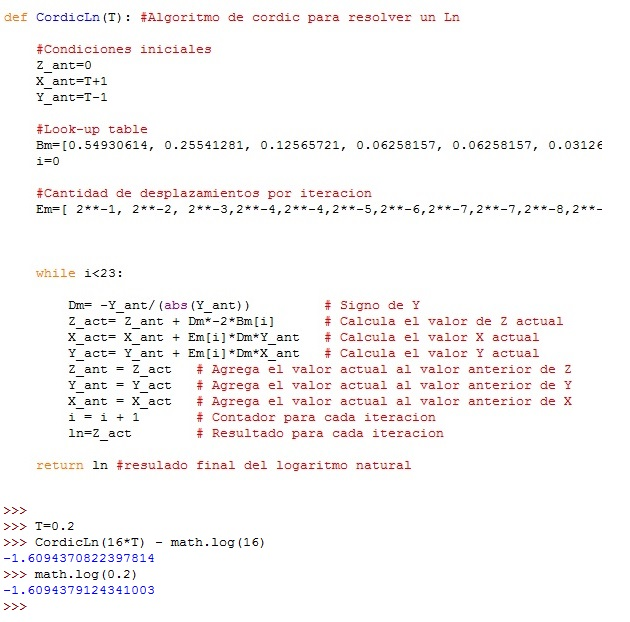
\includegraphics[scale=0.6]{./Progra_Cordic.jpg}
    \rule{35em}{0.5pt}
  \caption[Algoritmo de CORDIC en Python]{Algoritmo de CORDIC en Python  }
  \label{fig:Python}
\end{figure}


En la figura \ref{fig:Python} se observa el programa realizado para la verificación del algoritmo, para este se utilizan las ecuaciones del marco teórico descritas con anterioridad, también se comprueba el cambio en el rango de calculo con el escalado del argumento por 16. 

Para simplificar el diseño del hardware se realizan cambios en las ecuaciones originales, se cambia la resta del valor actual de Z por una suma, y se incluye el signo en la LUT de Z, el resultado final del algoritmo se debe multiplicar por 2, sin embargo este escalado se puede realizar en la LUT, esto para evitar la multiplicación, esto se comprueba en el programa de la figura \ref{fig:Python}.  


\section{Linealizador con el algoritmo de CORDIC}

\begin{figure}[H]
  \centering
    \includegraphics[scale=0.6]{./Linealizador_general.png}
    \rule{35em}{0.5pt}
  \caption[Bloque principal: algoritmo de CORDIC en hardware]{Bloque principal: Algoritmo de CORDIC en hardware  }
  \label{fig:CORDIC1}
\end{figure}

La figura \ref{fig:CORDIC1} contiene el bloque general del algoritmo de CORDIC, poseen 4 entradas: CLK , T , Begin\_LN , RST\_LN y 4 salidas: ACK\_LN , RESULT , U\_F , O\_F

\begin{figure}[H]
  \centering
    \includegraphics[scale=0.4]{./Linealizador_CORDIC_FSM.png}
    \rule{35em}{0.5pt}
  \caption[Coprocesador CORDIC y Control]{Coprocesador CORDIC y Control  }
  \label{fig:CORDIC2}
\end{figure}

El sistema de linealización de la figura \ref{fig:CORDIC2} cuenta con dos módulos principales: 

\begin{compactitem}

\item \nt{Coprocesador Cordic}: En este realizan todas las operaciones requeridas por el algoritmo, se encarga del manejo de los datos en el calculo. 


\item \nt{Control}: Este se encarga de proveer las señales de control requeridas por el coprocesador, según las condiciones que se tenga en cada estado.

\end{compactitem}

señales de datos: 

\begin{compactitem}

\item \nt{T}: Dato de entrada, argumento del logaritmo natural. 
\item \nt{RESULT}: Resultado de la operación logaritmo natural.

\end{compactitem}

señales de control: 

\begin{compactitem}
\item \nt{CLK}: Reloj del sistema. 

\item \nt{Begin\_LN}: Esta se encarga de dar inicio a la operación logaritmo natural. 

\item \nt{RST\_LN}: Realiza un reset a la unidad CORDIC tanto para el coprocesador como para la maquina de estados.
 

\item \nt{ACK\_LN}: Indica que el calculo ya fue realizado.

\item \nt{Begin\_SUM}: Esta se encarga de dar inicio a la unidad de suma-resta punto flotante.

\item \nt{ACK\_SUM}: Indica que esta listo el calculo realizado en la unidad de suma-resta punto flotante.

\item \nt{O\_F}: Indica si la suma-resta flotante realizada tiene un over-flow.

\item \nt{U\_F}: Indica si la suma-resta flotante realizada tiene un under-flow.

\item \nt{CLK\_DIR}: Activa el enable del contador de iteraciones. 

\item \nt{CONT\_ITER}: Indica el numero de iteracion, para que la maquina de estados pueda detenerse en el numero que se le asigne.
 
\item \nt{RST}: Realiza el reset de todos los registros de la unidad.

\item \nt{MS\_1 , MS\_2 , MS\_3 , MS\_4}: Realizan la selelccion de cada multiplexor, Mux1, Mux2, Mux3, Mux's4 respectivamente.

\item \nt{EN\_REG1X , EN\_REG1Y , EN\_REG1Z}: Activa los enable de los registros de la primera etapa REG1X, REG1Y, REG1Z respectivamente, para almacenar datos. 

\item \nt{EN\_REG2XYZ}: Activa el enable del registro REG2XYZ de la segunda etapa. 

\item \nt{EN\_REG2}: Activa el enable del registro REG2 de la segunda etapa.

\item \nt{EN\_REG3}: Activa el enable del registro REG3 del dato inicial.

\item \nt{EN\_REG4}: Activa el enable del registro REG4 del dato final. 

\end{compactitem}

\section{Coprocesador CORDIC}
El diseño de este algoritmo se basa en una arquitectura segmentada, de manera que se almacenan varios datos a la vez, sin embargo se debe tener buena sincronización para evitar datos erróneos a través del proceso de calculo. Por otro lado se utiliza el formato IEEE 754 con 32Bits, esto debido a que se requiere una adecuada precision en el calculo y un menor numero de iteraciones, repercutiendo en la velocidad del sistema. 

\begin{figure}[H]
  \centering
    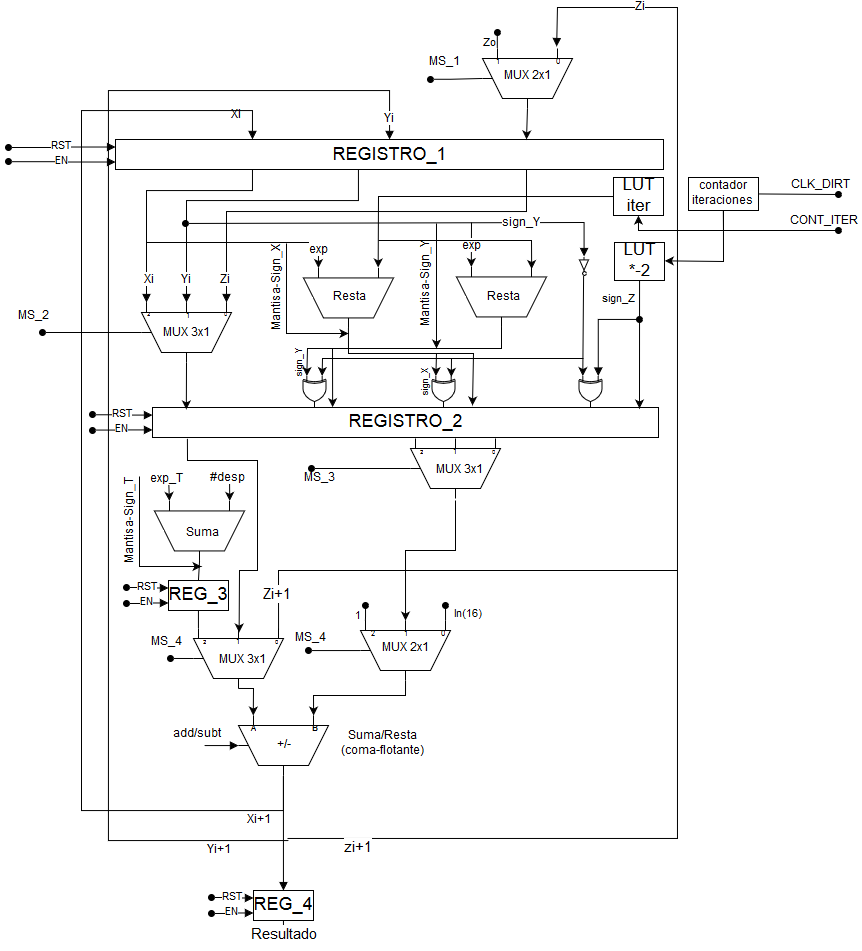
\includegraphics[scale=0.6]{./CORDICLN.png}
    \rule{35em}{0.5pt}
  \caption[Algoritmo de CORDIC en hardware]{Algoritmo de CORDIC en hardware  }
  \label{fig:CORDICLN}
\end{figure}

En la figura \ref{fig:CORDICLN} se puede observar la arquitectura diseñada para el algoritmo de CORDIC, con el formato IEEE 754 en 32-Bits, se trabaja en punto flotante, este reduce el numero de ieraciones, y produce una mejor precisión tanto en las operaciones como el resultado final. 

Esta etapa inicia con la carga de las condiciones iniciales, donde $\ Z_0 $ contiene un valor inicial cero, para el valor inicial de $\ X_0 $ y $\ Y_0 $ primeramente se aplica el escalado  16*T,
este escalado se puede representar como un desplazamiento $\ 2^{-4} $, por lo tanto este movimiento en punto flotante se traduce como una suma de 4 en el exponente de $\ T$, posteriormente se realizan las siguientes operaciones en punto flotante,  $\ X_0 = T + 1 $ y $\ Y_0 = T - 1 $, estas tres constantes dan inicio al proceso de calculo de manera iterativa, por lo que se requiere almacenarlas en un registro en la primera etapa de segmentación $\ \left(Registro 1 \right) $, los nuevos estados se deben calcular uno por uno, esto debido a que el circuito para el sumador-restador en punto flotante requiere de mucha área, este método (CORDIC) es un calculo cruzado es decir, para el próximo valor de $\ X_i$ se requiere un valor de $\ Y_0 $ con un desplazamiento y un cambio de signo, y para $\ Y_i $ se aplica un concepto similar con valores de $\ X_0$,  por lo tanto para el calculo de $\ X_i $ se requiere un restador en punto fijo para desplazar el valor del exponente de $\ Y_0 $ , para el nuevo valor de $\ Y_i $ se utiliza un restador punto fijo para el valor del exponente de $\ X_0 $ y para $\ Z_i $ se requiere una ROM con valores previamente cargados $\ \left(LUT \right) $. Estas operaciones "$\ X_i , Y_i $"  involucran el signo de "$\ Y_0 $" invertido.

Para el signo de las operaciones CORDIC se utiliza un circuito de comparación como se observa en la siguiente tabla: 

\begin{table}[H]
\centering
\caption{Tabla de signo para cada iteracion componente Xi , Yi , Zi}
\label{Table:Signo}
\begin{tabular}{|c|c|c|c|c|c|c|}
\hline
Sign $\ X_0 $ & Sign $\ Z_0 $  & Sign $\ Y_0 $ & Sign $\ \sim Y_0 $  & Sign $\ X_i $ & Sign $\ Z_i $  & Sign $\ Y_i $      \\ \hline

\begin{tabular}[c]{@{}c@{}} 0
\end{tabular}  & 0 & 0   & 1   & 1 & 1 & 1       \\ \hline

\begin{tabular}[c]{@{}c@{}} 0
\end{tabular} & 0 & 1   & 0  & 0 & 0 & 1       \\ \hline

\begin{tabular}[c]{@{}c@{}} 0 
\end{tabular} & 1 & 0   & 1 & 1 & 0 & 1\\ \hline
\begin{tabular}[c]{@{}l@{}} 0
\end{tabular} & 1 & 1   & 0  & 0 & 1 & 1   \\ \hline

\begin{tabular}[c]{@{}l@{}} 1
\end{tabular} & 0 & 0   & 1 & 0 & 1 & 1   \\ \hline

\begin{tabular}[c]{@{}l@{}} 1
\end{tabular} & 0 & 1   & 0  & 1 & 0 & 1   \\ \hline

\begin{tabular}[c]{@{}l@{}} 1
\end{tabular} & 1 & 0   & 1  & 0 & 0 & 1   \\ \hline

\begin{tabular}[c]{@{}l@{}} 1
\end{tabular} & 1 & 1   & 0 & 1 &  1 & 1    \\ \hline


\end{tabular}
\end{table}

\begin{figure}[H]
  \centering
    \includegraphics[scale=0.48]{./signo.png}
    \rule{35em}{0.5pt}
  \caption[Signo para cada iteración componente Xi , Yi , Zi]{Signo para cada iteración componente Xi , Yi , Zi   }
  \label{fig:SGN}
\end{figure}


A partir de la tabla \ref{Table:Signo} se extrae el circuito de comparación de signo de la figura \ref{fig:SGN}, este es diseñado con compuerta \nt{XOR} que poseen el mismo comportamiento de la tabla. 


Se requiere de dos Look-up tables "LUT", los datos de cada tabla se almacenan en memorias ROM's, de manera que puedan ser accesados en cualquier momento que sean requeridos, dentro de las ROM's se dispone:   

\begin{compactitem}

\item \nt{LUT\_Z}: Contiene almacenados los valores de $\ -2arctanh \left( 2^{-i} \right) $, para cada iteración.  
\item \nt{LUT\_ITER}: Esta contiene almacenados los desplazamientos que se deben realizar para cada iteración, esto debido a que las iteraciones 4 y 13 repiten desplazamientos como se menciona en el marco teórico. 

\end{compactitem}

El acceso a cada valor de la tablas se realiza mediante un contador de iteraciones, este indica a cada tabla la dirección que debe desplegar según el numero de iteración.  

El proceso para el calculo de las variables no se puede realizar de manera simultanea, ya que solo se cuenta con un sumador punto flotante, para esto se cuenta con las variables iniciales del registro 1 y se almacenan las variables modificadas en el \nt{Registro 2}, la secuencia de calculo toma primeramente los valores que se necesitan para el calculo de  $\ X_i $, posteriormente se realiza el calculo y se almacena el resultado en el \nt{Registro 1}, seguidamente se procede con el calculo de $\ Y_i $ y se almacena en el \nt{Registro 1}, por ultimo se calcula el valor de $\ Z_i $, concluida la suma se almacena en el \nt{Registro 1}, este proceso se hace de manera iterativa, una vez finalizada la cuenta de N iteraciones (Según se defina N=numero entero), se realiza la resta $\ Z_i - Ln\left(16\right) $ para contrarrestar el efecto del escalado aplicado al argumento$\ \left(T\right) $ al inicio del calculo del logaritmo natural, por ultimo el resultado final de $\ Z_i $ contiene el valor de $Ln \left(T \right)$ , este se almacena en el \nt{Registro 4}.

\section{Sistema de control para el coprocesador CORDIC}

\begin{figure}[H]
  \centering
    \includegraphics[scale=0.48]{./MaquinaL.png}
    \rule{35em}{0.5pt}
  \caption[Maquina de estados finitos para la arquitectura de CORDIC]{Maquina de estados finitos para la arquitectura de CORDIC   }
  \label{fig:FSML}
\end{figure}

EL sistema de control requiere de mucha sincronía, ya que los datos debe ser almacenados de manera correcta y estar listos cuando se requiere por otro segmento del coprocesador CORDIC, para esto se diseñó una maquina de estados finitos, donde inicialmente se calculan los valores iniciales de $ X_0 $, $ Y_0 $ y $ Z_0 $, posteriormente la maquina brinda las señales de control requeridas con la secuencia de calculo de $ X_i $,$ Y_i $ y $ Z_i $ respectivamente realizando una cuenta de iteración, se cuenta con una variable de entrada para que este control pueda saber el numero de iteración en el que se encuentra, de manera que cuando se llega a la iteración N definida con anterioridad, se finaliza el calculo.

\section{Algoritmo de CORDIC en Verilog}

Este algoritmo se implementó por medio de el lenguaje de descripción de hardware "Verilog", inicialmente se realizaron pequeños bloques pertenecientes a cada elemento requerido por la arquitectura diseñada, se vio la necesidad, por cuestión de orden, de desarrollar el coprocesador CORDIC y la unidad de control en bloques separados, de manera que se pudieran realizar pruebas sin dependencia de los bloques entre si, para una mejor depuración de errores y re-diseño. Finalmente se realizan las simulaciones al bloque completo en la figura \ref{fig:SIMLINEAL}. 

\begin{figure}[H]
  \centering
    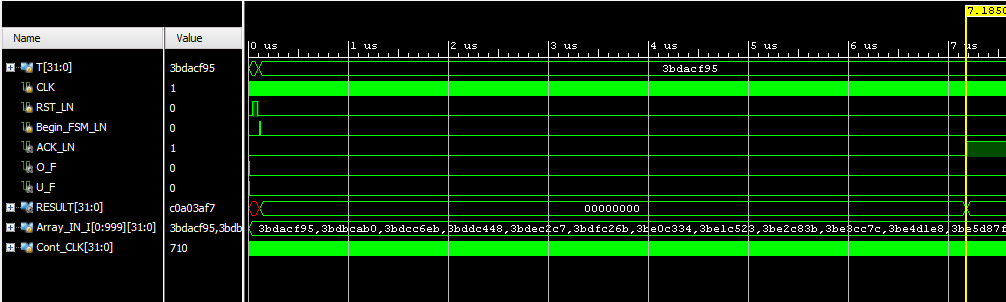
\includegraphics[scale=0.6]{./TEST_LINEALIZADOR_I.png}
    \rule{35em}{0.5pt}
  \caption[Simulación del linealizador en implementado en Verilog]{Simulación del linealizador en implementado en Verilog}
  \label{fig:SIMLINEAL}
\end{figure}   

\section{Simulación del algoritmo de CORDIC}

Las simulaciones de la implementación del algoritmo, se realizaron mediante mil valores de entrada, obteniendo así mil valores de salida, los cuales se comparan con los valores reales, para dicha comparación se realizaron aproximaciones con 8, 12 y 15 iteraciones. 

Primeramente se realiza una simulación que comprueba el funcionamiento en el rango de operación $\ 0.00667769 < T < 0.58496687 $ y la linealización esta prueba se realiza con la siguiente función: 

\begin{equation} \label{eq:ej2}
  Ln \left(T \right) 
\end{equation} 

donde el argumento T es:

\begin{equation} \label{eq:ej3}
   T = e^{-x}         
\end{equation} 
  
El intervalo $\ 0,536 < x < 5,009$ se divide en mil valores, de manera que la función \ref{eq:ej2} devuelve mil valores, estos se almacenan en un archivo .txt de manera que se insertan en el circuito CORDIC para obtener mil valores del cálculo. 


\begin{equation} \label{eq:ej4}
   V_{pv} = V_{cte} + 0.3*V_{cte}*sin(2* \pi *100*t)     
\end{equation}


    
\begin{equation} \label{eq:ej5}
   i_{pv} = Ig - \frac{V_{pv}}{R_p} - Is*\left(e^\frac{V_{pv}* \alpha}{2}\right)         
\end{equation} 


Seguidamente se realiza una prueba con mil valores simulando el comportamiento que tiene un PV, utilizando el modelo del panel, donde se utiliza el valor de $ V_{pv} $ para cada valor de tiempo, en la ecuación \ref{eq:ej5} obteniendo valores de corriente de entrada $ i_{pv} $ para el linealizador, así poder observar si se realiza la linealización en la salida. 



\subsection{Simulacion del rango de convergencia del Linealizador CORDIC}

En la implementación de un algoritmo en hardware, es de suma importancia verificar que este funcione de manera adecuada en el rango de convergencia definido. Para la comprobación del algoritmo de la unidad del linealizador CORDIC, se realizaron una serie de pruebas, simulando con cierta cantidad de iteraciones y así poder observar cual es la mas adecuada para el calculo requerido y su debido resultado, para esto se programó un simulación("testbench") en donde se corre una prueba con mil valores de entrada, ingresados por medio de un archivo de texto previamente editado con los datos de entrada con la función exponencial anteriormente descrita en la ecuación \ref{eq:ej3}. 


\begin{figure}[H]
  \centering
    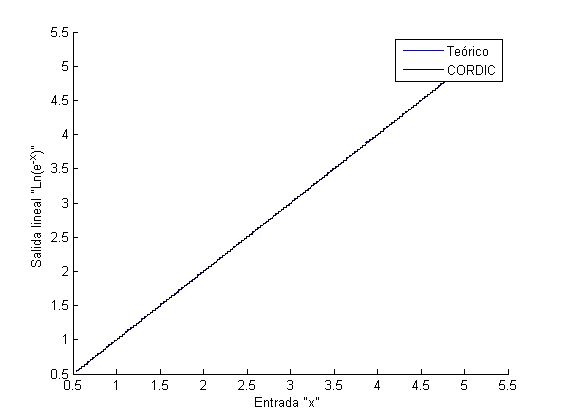
\includegraphics[scale=0.7]{./RANGO_8iter.png}
    \rule{35em}{0.5pt}
  \caption[Rango de convergencia circuito CORDIC con 8 iteraciones]{Rango de convergencia circuito CORDIC con 8 iteraciones   }
  \label{fig:RG8}
\end{figure}

\begin{figure}[H]
  \centering
    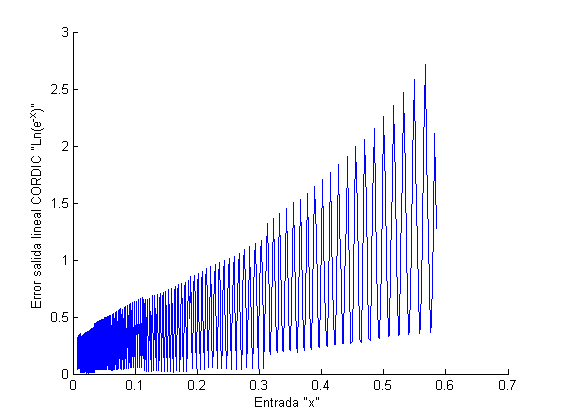
\includegraphics[scale=0.7]{./RANGO_8iter_ERROR.png}
    \rule{35em}{0.5pt}
  \caption[\%Error rango de convergencia circuito CORDIC con 8 iteraciones]{\%Error rango de convergencia circuito CORDIC con 8 iteraciones }
  \label{fig:RGE8}
\end{figure}


Primeramente se realizó una simulación con 8 iteraciones, como se muestra en la figura \ref{fig:RG8}, para el cálculo de cada valor se requieren 460 ciclos de reloj desde el momento en se activa la señal Begin\_LN hasta que se recibe la señal ACK\_LN, que es donde se indica que se ha completado el cálculo, es de suma importancia realizar la comparación entre el valor teórico y el valor calculado obtenido. Para cada valor se calculó el error, estos se pueden observar en la figura \ref{fig:RGE8}, donde el porcentaje de error máximo es de 2,72\% y el porcentaje de error promedio es de 0,40\%. 
 




\begin{figure}[H]
  \centering
    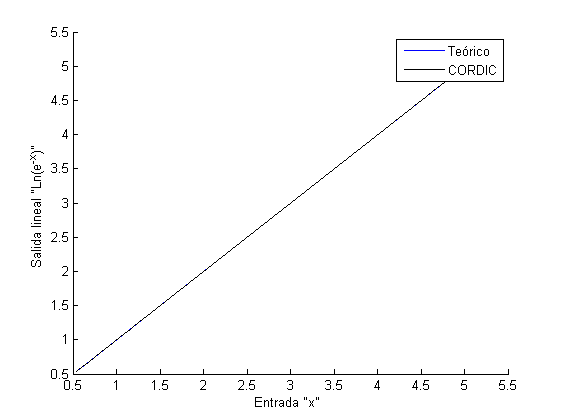
\includegraphics[scale=0.7]{./RANGO_12iter.png}
    \rule{35em}{0.5pt}
  \caption[Rango de convergencia circuito CORDIC con 12 iteraciones]{Rango de convergencia circuito CORDIC con 12 iteraciones   }
  \label{fig:RG12}
\end{figure}

\begin{figure}[H]
  \centering
    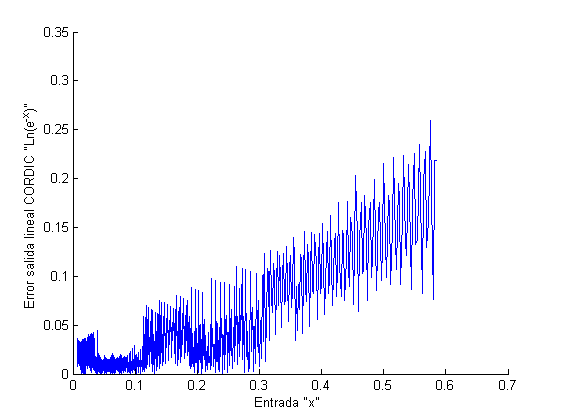
\includegraphics[scale=0.7]{./RANGO_12iter_ERROR.png}
    \rule{35em}{0.5pt}
  \caption[\%Error rango de convergencia circuito CORDIC con 12 iteraciones]{\%Error rango de convergencia circuito CORDIC con 12 iteraciones }
  \label{fig:RGE12}
\end{figure}

Una mejor aproximación se puede lograr utilizando 12 iteraciones en el calculo del logaritmo natural, en la figura \ref{fig:RG12} se pueden observar los resultados obtenidos, se requieren 675 ciclos de reloj para ejecutar el cálculo completo. La figura \ref{fig:RGE12} muestra el error en cada cálculo, donde el porcentaje de error máximo es de  0,259\% y el porcentaje de error promedio es de 0,0351\%. 

\begin{figure}[H]
  \centering
    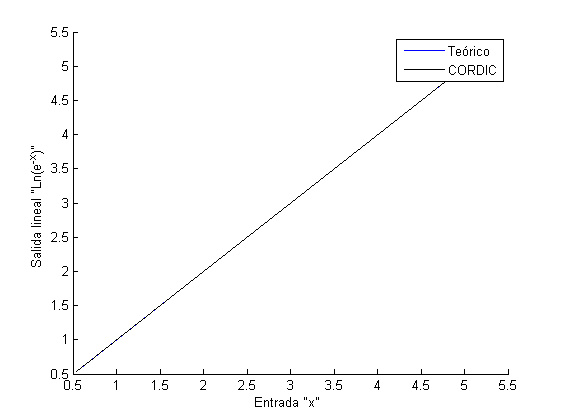
\includegraphics[scale=0.7]{./RANGO_15iter.png}
    \rule{35em}{0.5pt}
  \caption[Rango de convergencia circuito CORDIC con 15 iteraciones]{Rango de convergencia circuito CORDIC con 15 iteraciones   }
  \label{fig:RG15}
\end{figure}

\begin{figure}[H]
  \centering
    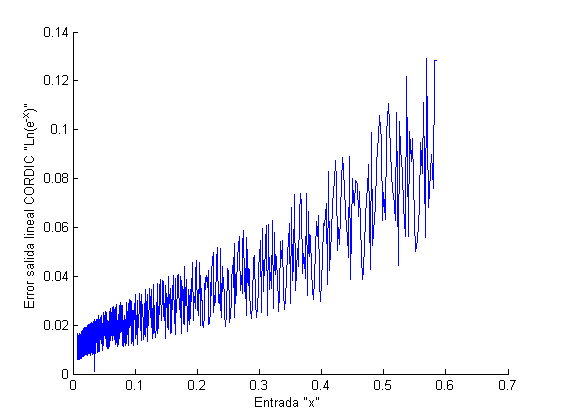
\includegraphics[scale=0.7]{./RANGO_15iter_ERROR.png}
    \rule{35em}{0.5pt}
  \caption[\%Error rango de convergencia circuito CORDIC con 15 iteraciones]{\%Error rango de convergencia circuito CORDIC con 15 iteraciones }
  \label{fig:RGE15}
\end{figure}


Utilizando 12 iteraciones en el cálculo del logaritmo natural se logra la mayor aproximación, sin embargo se requieren 818 ciclos de reloj y se vuelve mas lento el proceso, en la figura \ref{fig:RG15} se pueden observar los resultados obtenidos. La figura \ref{fig:RGE15} muestra el error en cada cálculo, donde el porcentaje de error máximo es de  0,129\% y el porcentaje de error promedio es de 0,0257\%. 



    